\documentclass[12pt,a4paper,bibliography=totocnumbered,listof=totocnumbered]{scrartcl}
% u.U. muss Koma-Skript Package ueber MikTeX deinstalliert und neu installiert werden
% Hilft das nicht, so sollte statt scrartcl die Dokumentenklasse article verwendet werden
%\usepackage[backend=bibtex,style=alphabetic]{biblatex}
%\usepackage[backend=bibtex,style=ieee]{biblatex}
\usepackage[style=ieee]{biblatex}
\usepackage[ngerman]{babel}
\usepackage[utf8]{inputenc}
\usepackage{ifthen}
\usepackage{xargs}
\usepackage{amsmath}
\usepackage{amsfonts}
\usepackage{amssymb}
\usepackage{graphicx}
\usepackage{caption}
\usepackage{fancyhdr}
\usepackage{tabularx}
\usepackage{geometry}
\usepackage{setspace}
\usepackage[right]{eurosym}
\usepackage[printonlyused]{acronym}
\usepackage{subfig}
\usepackage{floatflt}
\usepackage[usenames,dvipsnames]{color}
\usepackage{colortbl}
\usepackage{paralist}
\usepackage{array}
\usepackage{titlesec}
\usepackage{parskip}
\usepackage[right]{eurosym}
\usepackage[subfigure,titles]{tocloft}
%\usepackage[pdfpagelabels=true]{hyperref}
\usepackage[pdfpagelabels=true]{hyperref}

\usepackage{listings}
\lstset{basicstyle=\footnotesize, captionpos=b, breaklines=true, showstringspaces=false, tabsize=2, frame=lines, numbers=left, numberstyle=\tiny, xleftmargin=2em, framexleftmargin=2em}
\makeatletter
\def\l@lstlisting#1#2{\@dottedtocline{1}{0em}{1em}{\hspace{1,5em} Lst. #1}{#2}}
\makeatother

%\geometry{a4paper, top=27mm, left=20mm, right=20mm, bottom=35mm, headsep=10mm, footskip=12mm}

\definecolor{javared}{rgb}{0.6,0,0} % for strings
\definecolor{javagreen}{rgb}{0.25,0.5,0.35} % comments
\definecolor{javapurple}{rgb}{0.5,0,0.35} % keywords
\definecolor{javadocblue}{rgb}{0.25,0.35,0.75} % javadoc
\definecolor{gray}{rgb}{0.6,0.6,0.6}
 
\lstset{language=Java,
basicstyle=\ttfamily\footnotesize,
keywordstyle=\color{javapurple}\bfseries,
stringstyle=\color{javared},
commentstyle=\color{javagreen}\itshape\bfseries,
morecomment=[s][\color{javadocblue}]{/**}{*/},
numbers=left,
numberstyle=\tiny\color{gray},
stepnumber=1,
numbersep=10pt,
tabsize=3,
showspaces=false,
showstringspaces=false}
\titlespacing{\section}{0pt}{12pt plus 4pt minus 2pt}{-6pt plus 2pt minus 2pt}

% Kopf- und Fusszeile
\renewcommand{\sectionmark}[1]{\markright{#1}}
\renewcommand{\leftmark}{\rightmark}
\pagestyle{fancy}
\lhead{}
\chead{}
\rhead{\thesection\space\contentsname}
\lfoot{}
\cfoot{}
\rfoot{\ \linebreak Seite \thepage}
\renewcommand{\headrulewidth}{0.4pt}
\renewcommand{\footrulewidth}{0.4pt}

% Vorspann
\renewcommand{\thesection}{\Roman{section}}
\renewcommand{\theHsection}{\Roman{section}}
\pagenumbering{Roman}

\newcommand{\folgen}[1]{
\ensuremath
#1
}

\newcommandx{\student}[3][]{
	\def\studentName{#1}%
	\def\studentMatnr{#2}%
	\def\studentStudiengang{#3}%
}

\newcommandx{\MyTitelseite}[8][]{
\thispagestyle{empty}

\includegraphics[scale=0.2]{pics/oth-logo.png}%\hfill\includegraphics[scale=0.5]{#1}
\begin{center}
\ifthenelse{\equal{#2}{2}}{ % then
	\vspace*{2cm}
	\Large
	\textbf{Ostbayerische Technische Hochschule Regensburg}\\
	\textbf{Fakultät für Informatik und Mathematik}\\
	\vspace*{2cm}
	\Huge
	\textbf{#3}\\[1em]
	\large
	Zur Erlangung des akademischen Grades des\\
	\ifthenelse{\equal{#3}{Bachelorarbeit}}{Bachelor of Science (B.Sc.)}{Master of Science (M.Sc.)}\\
	\vspace*{1cm}
	\Large
	\textbf{#4}\\
}{ % else
	\vspace*{1cm}
	\Large
	\textbf{#4}\\
	\vspace*{2cm}
	\large
	An der Fakultät für Informatik und Mathematik der\\
	Ostbayerischen Technischen Hochschule Regensburg\\
	im Studiengang\\
	\studentStudiengang\\[2em]
	eingereichte\\
	\vspace*{1cm}
	\Large
	\textbf{#3}\\[2em]
	\large
	zur Erlangung des akademischen Grades des\\
	\ifthenelse{\equal{#3}{Bachelorarbeit}}{Bachelor of Science (B.Sc.)}{Master of Science (M.Sc.)}
	\vspace*{1cm}
	\Large
}
	\vfill
	\normalsize
	%\newcolumntype{x}[1]{>{\raggedleft\arraybackslash\hspace{0pt}}p{#1}}
	\begin{tabular}{rl}%{6cm}p{7.5cm}}
	    \rule{0mm}{1ex}\textbf{Vorgelegt von:} & \studentName \\
		\rule{0mm}{1ex}\textbf{Matrikelnummer:} & \hspace*{-0.5em}\begin{tabular}[t]{r}\studentMatnr\end{tabular} \\ 
		\ifthenelse{\equal{#2}{1}}{~\\}{\rule{0mm}{1ex}\textbf{Studiengang:} & \studentStudiengang \\[2em]}
		\rule{0mm}{1ex}\textbf{Erstgutachter:} & #5 \\ 
		\rule{0mm}{1ex}\textbf{Zweitgutachter:} & #6 \\[2em]
		\rule{0mm}{1ex}\textbf{Abgabedatum:} & #7 \\ 
	\end{tabular} 
\end{center}
\pagebreak
}
%\addbibresource{literatur.bib}
\addbibresource{mendeley.bib}


\begin{document}


% ----------------------------------------------------------------------------------------------------------
% Titelseite
% ----------------------------------------------------------------------------------------------------------
\newcommand{\studierenderName}{Philipp Gottschalk}
\student{\studierenderName}		% Studierender
{2853044}						% Matrikelnummer
{Technische Informatik}			% Studiengang

\MyTitelseite{}	% Optionales Logo des extern betreuenden Unternehmens
{1}								% Style der Titelseite (1 oder 2)
{Bachelorarbeit}				% Typ der Abschlussarbeit (\in {Bachelorarbeit, Masterarbeit})
{Analyse und Vergleich von Prozess-Isolationsmechanismen bei Containern und Virtuellen Maschinen}				% Thema der Arbeit						
{Prof.\ Dr.\ Alexander Metzner}		% Betreuer
{Prof.\ Dr.\ Richard Roth}	% Zweitgutachter
{13.10.\the\year}				% Abgabedatum


\thispagestyle{empty}
~\pagebreak

\setcounter{page}{1} 

% ----------------------------------------------------------------------------------------------------------
% Eigensctändigkeitserklaerung
% ----------------------------------------------------------------------------------------------------------
\thispagestyle{empty}
\section*{Erklärung zur Bachelorarbeit}

\bigskip
\bigskip 
\bigskip 

\begin{enumerate}
    \item Mir ist bekannt, dass dieses Exemplar der Bachelorarbeit als Prüfungsleistung in das Eigentum der Ostbayerischen Technischen Hochschule Regensburg übergeht.
    \item Ich erkläre hiermit, dass ich diese Bachelorarbeit selbständig verfasst, noch nicht anderweitig für Prüfungszwecke vorgelegt, keine anderen als die angegebenen Quellen und Hilfsmittel benutzt sowie wörtliche und sinngemäße Zitate als solche gekennzeichnet habe.
\end{enumerate}

\bigskip 
\bigskip 
\bigskip 

Regensburg, den \today

\bigskip 
\bigskip

\line(1,0){200}
\newline
\studierenderName

% ----------------------------------------------------------------------------------------------------------
% Abstract
% ----------------------------------------------------------------------------------------------------------
\thispagestyle{empty}
\setstretch{1.15} % Zeilenspacing
\section*{Zusammenfassung}

\bigskip 


In der folgenden Arbeit wird $\ldots$


% ----------------------------------------------------------------------------------------------------------
% Inhaltsverzeichnis
% ----------------------------------------------------------------------------------------------------------
\tableofcontents
\pagebreak

% ----------------------------------------------------------------------------------------------------------
% Abbildungsverzeichnis
% ----------------------------------------------------------------------------------------------------------
\lhead{}
\rhead{Abbildungsverzeichnis}
\listoffigures
\pagebreak

% ----------------------------------------------------------------------------------------------------------
% Tabellenverzeichnis (optional)
% ----------------------------------------------------------------------------------------------------------
\lhead{}
\rhead{Tabellenverzeichnis}
\listoftables
\pagebreak

% ----------------------------------------------------------------------------------------------------------
% Listingsverzeichnis (optional; Code nur, wenn wirklich sinnvoll und wichtig)
% ----------------------------------------------------------------------------------------------------------
%\lhead{}
%\rhead{Quellcodeverzeichnis}
%\lstlistoflistings
%\pagebreak

% ----------------------------------------------------------------------------------------------------------
% Abkürzungsverzeichnis (optional)
% ----------------------------------------------------------------------------------------------------------
\lhead{}
\rhead{Abkürzungsverzeichnis}
%\listoftables
\section{Abkürzungsverzeichnis}
\begin{acronym}[KDE]
\acro{BA}[BA]{Bachelorarbeit}
\acro{MA}[MA]{Masterarbeit}
\end{acronym}
\pagebreak


% ----------------------------------------------------------------------------------------------------------
% Inhalt
% ----------------------------------------------------------------------------------------------------------
% Abstände Überschrift
\titlespacing{\section}{0pt}{12pt plus 4pt minus 2pt}{0pt plus 2pt minus 2pt}
\titlespacing{\subsection}{0pt}{12pt plus 4pt minus 2pt}{0pt plus 2pt minus 2pt}
\titlespacing{\subsubsection}{0pt}{12pt plus 4pt minus 2pt}{0pt plus 2pt minus 2pt}
%\titlespacing{\subsubsubsection}{0pt}{12pt plus 4pt minus 2pt}{0pt plus 2pt minus 2pt}
% Kopfzeile
\renewcommand{\sectionmark}[1]{\markright{#1}}
\renewcommand{\subsectionmark}[1]{}
\renewcommand{\subsubsectionmark}[1]{}
%\renewcommand{\subsubsubsectionmark}[1]{}

\lhead{Kapitel \thesection}
\rhead{\rightmark}

%\onehalfspacing
\setstretch{1.15}
\renewcommand{\thesection}{\arabic{section}}
\renewcommand{\theHsection}{\arabic{section}}
\setcounter{section}{0}
\pagenumbering{arabic}
\setcounter{page}{1}

% ----------------------------------------------------------------------------------
% Kapitel: Einleitung
% ----------------------------------------------------------------------------------
\section{Einleitung}
\subsection{Motivation}
\subsection{Projektbeschreibung}
\subsection{Ziele}
Sie können dieses \LaTeX-Template als Vorlage für Ihre Abschlussarbeit (\ac{BA}, \ac{MA}) nutzen und auf Wunsch natürlich auch selbstständig erweitern. Auf den folgenden Seiten finden Sie einige Hinweise zu \LaTeX. Sollten Sie Fragen haben, wenden Sie sich gerne an mich unter: \url{carsten.kern@oth-regensburg.de} 



\pagebreak
% ----------------------------------------------------------------------------------
% Kapitel: Theorie
% ----------------------------------------------------------------------------------
\section{Theorie}
\subsection{Container}
Container-basierte Virtualisierung ist ein leichtgewichtiger Virtualisierungsansatz auf Betriebssystemebene, bei dem der Host-Kernel zur Ausführung mehrerer virtueller Umgebungen verwendet wird. Diese virtuellen Umgebungen werden oft einfach als \glqq Container \grqq{} bezeichnet. Linux-V Server[X], Open VZ\cite{IndexOpenvz.org} und Linux Container(LXC)\cite{IndexLinuxcontainers.Org} sind die drei wichtigsten Vertreter dieses Ansatzes. Die allgemeine Architektur einer Container-basierten Virtualisierungslösung ist in (Abb1) dargestellt. Containerbasierte Virtualisierung erfolgt auf Betriebssystem Ebene, so dass mehrere Anwendungen ohne redundante Ausführung anderer Betriebssystem Kerne auf dem Host betrieben werden können. Container sehen von außen aus wie normale Prozesse, die auf dem Kernel laufen, der mit dem Host-Rechner geteilt wird. Sie stellen eine isolierte Umgebung mit den notwendigen Ressourcen für die Ausführung von Anwendungen zur Verfügung. Diese Ressourcen können entweder mit dem Host geteilt oder separat im Container installiert werden \cite{Xavier2014AClusters}. Namespaces sind die Basis des LXC und stellen in Verbindung mit anderen Ressourcen-Management-Systemen eine isolierte Umgebung in Form von Containern zu Verfügung. LXC nimmt die cgroups Ressourcenverwaltungseinrichtungen\cite{ControlDocumentation} als Grundlage und fügt POSIX file Fähigkeiten [X] hinzu, um die Ressourcen unter den Containern einzuschränken. 

\vspace{1em}
\begin{minipage}{\linewidth}
	\centering
	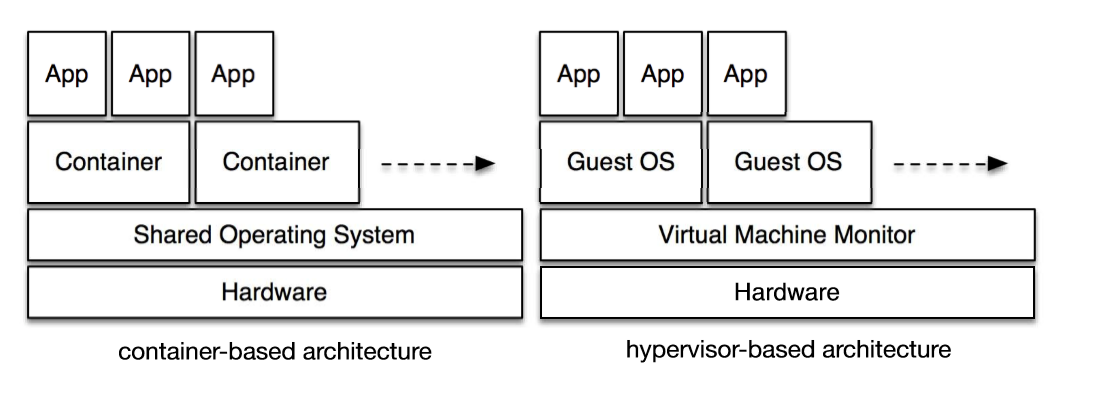
\includegraphics[width=1\linewidth]{pics/docker2.png}
	\captionof{figure}[Abbildung1]{Aufbau Container und Virtuelle Maschine \cite{Xavier2015AClouds}}
	\label{fig:reversi2}
\end{minipage}


\subsection{Virtuelle Maschine}
Typ-2-Hypervisor-basierte Virtualisierung erstellt eine komplette virtuelle Maschine auf dem Host Betriebssystem(Abb1). Jede virtuelle Maschine besteht nicht nur aus einer Anwendung mit ihren Abhängigkeiten, sondern aus einem kompletten Gastbetriebssystem und einem separaten Kernel. Es gibt zwei Klassen von Hypervisoren: den Typ-1-Hypervisor, auch bekannt als "Bare-Metal-Hypervisor", der direkt auf der zugrundeliegenden Hardware des Hosts arbeitet, und dem Typ-2-Hypervisor, auch bekannt als der "gehostete Hypervisor", der auf dem Host-Betreibssystem arbeitet.

\subsubsection{Typ1-Hypervisor}
Typ-1-Hypervisor-basierte (Bare Matal Hypervisor)
\subsubsection{Typ2-Hypervisor}


\subsection{Isolation}
Das Ziel der Prozessisolation ist es, zu verhindern, dass Container untereinander beeinflussbar sind. Dieses Unterfangen ist mit Hilfe der sogenannten "namespaces" möglich. 

-Resourcenisolation 

\subsubsection{Kernel-Namespaces}
Mit Hilfe der Namespaces kann man die Prozessisolation zwischen den Containern sicher stellen. Ein Container kann nur seine Eigenen Ressourcen sehen.

\paragraph{PID-Namespace} ist hierarchisch[X] deshalb kann ein Prozess nur die anderen Prozesse in seinem eigenen Namensraum oder in seinen untergeordneten Namensräumen sehen. Folglich kann der Host die Prozesse innerhalb des neuen PID-namespace des Containers beobachten und beeinflussen, aber die Prozesse innerhalb des Containers können die anderen Prozesse, die im Host oder in anderen Containern laufen, nicht beobachten oder beeinflussen

\paragraph{Mount-Namespace} isoliert filesystem Mountpunkte, die von einem Container gesehen werden, so dass Prozesse in verschiedenen Containerern unterschiedliche Ansichten der file Systemhierarchie haben können.

\paragraph{UTS-Namespace} erlaubt es jedem Container seinen eigenen Hostnamen und NIS-Domänennamen zu haben.

\paragraph{IPC-Namespace} isoliert die Interprozesskommunikation, das bedeutet Prozesse, die in einem Container enthalten sind, haben eigene Nachrichten Warteschlangen und sind völlig unabhängig von Prozessen in anderen Containern.

\paragraph{Network namespace} isoliert das Netzwerk-Untersystem wie z.B. Geräte und IP-Adressen. Jeder Container unterhält seine eigene Netzwerk Configuration und die darauf laufenden Anwendung.

\paragraph{User-Namespace} isoliert Benutzer-IDs vom Host und anderen laufenden Containern. Das bedeutet, dass der Benutzer root (ID0) innerhalb eines Containers volle Privilegien hat, aber keine Privilegien außerhalb, was Sicherheit und Zuverlässigkeit gewährleistet. \cite{Xavier2015AClouds}
	



\subsubsection{cgroup}
\glqq c-group\grqq{} steht für \glqq contol group\grqq{}. Durch cgroup ist es möglich, eine Reihe von Kriterien anzuwenden, um Ressourcen wie Speicher,Netzwerk, Festplatten-I/O und CPU einzuschränken. Ein Container sollte seine auferlegten Beschränkungen nicht überschreiten und andere Container, die auf derselben Hardware laufen, nicht stören. Cgroup ist für die Ressourcen Begrenzung, Priorisierung, Abrechnung und Kontrolle zuständig.\cite{Heo2015ControlV2}



\paragraph{Speicher}



\subsubsection{POSIX file capabilitie}
%\subsubsection{adds POSIX file capabilitie}

\subsubsection{VMM}

\paragraph{test}

\pagebreak

 ----------------------------------------------------------------------------------
% Kapitel: Praktische Umsetzung
% ----------------------------------------------------------------------------------
\section{Praktische Durchführung}
\subsection{Hardware}
\subsection{Docker}
\subsection{Realisierung}
\subsection{Ergebnis}


\pagebreak

% ----------------------------------------------------------------------------------
% Kapitel: Fazit und Ausblick
% ----------------------------------------------------------------------------------
\section{Fazit und Ausblick}



\pagebreak
% ----------------------------------------------------------------------------------
% Kleine Einführung in LaTeX-Elemente
% ----------------------------------------------------------------------------------
\section{\LaTeX-Elemente}
Dieser Abschnitt beinhaltet lediglich einige Informationen über \LaTeX-Distributionen, Editoren und \LaTeX-Elemente, die Ihnen beim Einstieg in das \LaTeX-Textsatzsystem helfen sollen.

\subsection{\LaTeX-Distributionen nach Betriebssystemen}

\subsubsection{\LaTeX-Distributionen}
Folgende Haupt-\LaTeX-Distributionen stehen Ihnen zur Verfügung:
\begin{itemize}
  \item Windows:\quad \texttt{MiKTeX}\quad Webseite:\quad\url{http://www.miktex.org}
  \item Linux/Unix:\quad \texttt{TeX Live}\quad Webseite:\quad\url{http://tug.org/texlive/}
  \item Mac OS:\quad \texttt{MacTeX}\quad Webseite:\quad\url{http://www.tug.org/mactex/}
\end{itemize}

\subsubsection{\LaTeX-Editoren}
Auf folgenden Webseiten können Sie einige hilfreiche \LaTeX-Editoren finden:
\begin{itemize}
  \item Windows/Linux/Mac OS: \url{http://www.xm1math.net/texmaker/}
  \item Windiws: \url{http://www.texniccenter.org/}
  \item Mac OS: \url{http://pages.uoregon.edu/koch/texshop/}
\end{itemize}

Falls bei den oben genannten Editoren kein passender vorhanden war, findet sich auf Wikipedia eine Zusammenstellung vieler weiterer \LaTeX-Editoren:\\[1em]
\hspace*{3cm}\url{https://en.wikipedia.org/wiki/Comparison_of_TeX_editors}


\subsection{Bilder}
Zum Einfügen eines Bildes, siehe Abbildung \ref{fig:reversi01}, werden die \texttt{minipage}-Umgebung und der Befehl \texttt{$\backslash$includegraphics} genutzt, da die Bilder so gut positioniert und einfach integriert und skaliert werden können.

\vspace{1em}
\begin{minipage}{\linewidth}
	\centering
	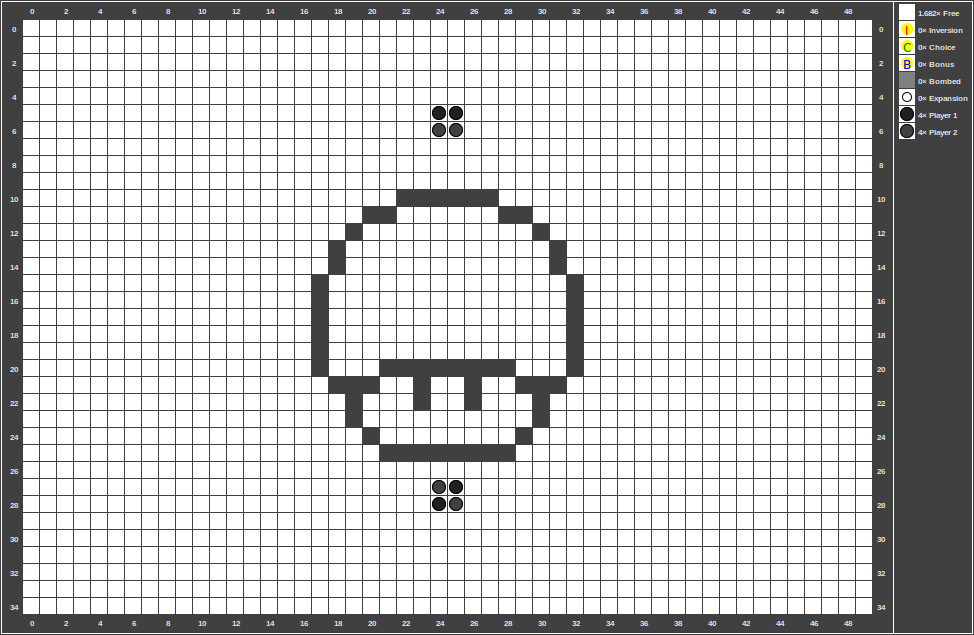
\includegraphics[width=0.5\linewidth]{pics/gamefield01.png}
	\captionof{figure}[Spielfeld 01]{Unbespieltes Spielfeld\footnotemark }
	\label{fig:reversi01}
\end{minipage}
\footnotetext{Diesem Spielfeld wurden noch keine Spieler zugewiesen (daher die dunklen Spielsteine)}

Nachdem das Spielt gestartet wurde und beide Spielphasen durchlaufen wurden, siegt schließlich der Spieler mit der Farbe rot.

%\vspace{1em}
%\begin{minipage}{\linewidth}
%	\centering
%	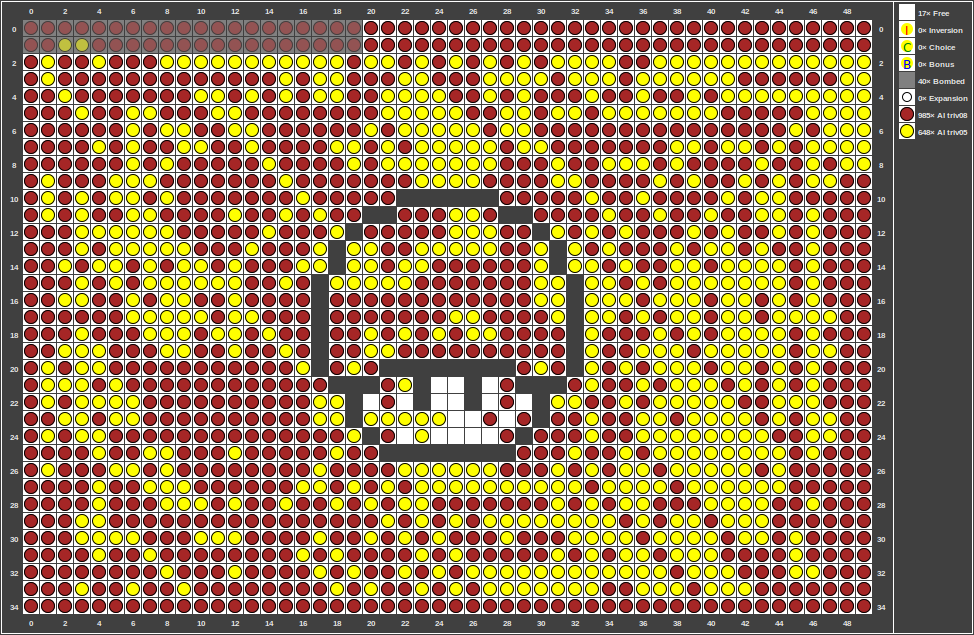
\includegraphics[width=0.5\linewidth]{pics/gamefield02.png}
%	\captionof{figure}[Spielfeld 02]{Finales Spielfeld\footnotemark }
%	\label{fig:reversi2}
%\end{minipage}
%\footnotetext{Das Spielfeld nach der Zug- und Bombenphase. Spieler rot gewinnt eindeutig.}

\subsection{Tabellen}
In diesem Abschnitt wird eine Tabelle (siehe Tabelle \ref{tab:beispiel}) dargestellt.

\vspace{1em}
\begin{table}[!h]
	\centering
	\begin{tabular}{|l|l|l|}
		\hline
		\textbf{Name} & \textbf{Name} & \textbf{Name}\\
		\hline
		1 & 2 & 3\\
		\hline
		4 & 5 & 6\\
		\hline
		7 & 8 & 9\\
		\hline
	\end{tabular}
	\caption{Beispieltabelle}
	\label{tab:beispiel}
\end{table}


\subsection{Auflistung}
Für Auflistungen wird die \texttt{enumerate}- oder \texttt{itemize}-Umgebung genutzt.

\begin{itemize}
	\item Nur
	\item ein
	\item Beispiel.
\end{itemize}

\subsection{Listings}
Zuletzt sehen Sie in Listing \ref{lst:maxTeilsumZweiD} ein Beispiel für das Einbinden von Quellcode mit Syntax-Highlighting.

\vspace{1em}
\lstinputlisting[caption=Brute Force-Ansatz für das MaxTeilsum2D-Problem, label=lst:maxTeilsumZweiD,basicstyle=\ttfamily\scriptsize]{code/maxTeilsum2DBruteForce.txt}

\subsection{Selbstgestaltete Abbildungen}
Mithilfe des Paketes \texttt{tikz} können sehr schöne Abbildungen (z.\,B.\ Automaten, Graphen etc.) direkt in \LaTeX generiert werden. Viele Beispiele dazu finden Sie auf folgender Webseite:\\[1em]
\hspace*{3cm}\url{http://www.texample.net/tikz/}.

\subsection{Tipps}
Die Literaturreferenzen (Bücher, Paper und Journals) und Internetquellen (Webseiten, Blogs etc.) befinden sich in der Datei \textit{literatur.bib}. Eine Buch- und eine Online-Quelle sind beispielhaft eingefügt.  %\cite{Bui2015AnalysisSecurity} 

Literatur und Quellen werden in zwei getrennte Verzeichnisse aufgeteilt. Als Unterscheidungsmerkmal dient bei den Quellen der Zusatz: \texttt{keywords = \{online\}}.

\pagebreak

% ----------------------------------------------------------------------------------------------------------
% Filter fuer Literatur und Quellen definieren
% ----------------------------------------------------------------------------------------------------------

%\defbibheading{Literatur}{\section*{Literaturverzeichnis}} 
\defbibheading{Quellen}{\section*{Quellenverzeichnis}} 
  
%\defbibfilter{Literatur}{\not\keyword{online}} 
%\defbibfilter{Quellen}{\keyword{online}} 


% ----------------------------------------------------------------------------------------------------------
% Literatur
% ----------------------------------------------------------------------------------------------------------
%\lhead{} 
%\rhead{Literaturverzeichnis} 

%\printbibliography[heading=Literatur,filter=Literatur] 

%\pagebreak


% ---------------------------------------------------------------------------------------------------------- 
% Quellen 
% ---------------------------------------------------------------------------------------------------------- 
\lhead{} 
\rhead{Quellenverzeichnis} 

%\printbibliography[title = {Quellenverzeichnis}, heading=Quellen] 
%\printbibliography[title = {Quellenverzeichnis},
\printbibliography[title = {Quellenverzeichnis}, heading=Quellen]

\pagebreak 

% ----------------------------------------------------------------------------------------------------------
% Anhang
% ----------------------------------------------------------------------------------------------------------
\pagenumbering{Roman}
\setcounter{page}{1}
\lhead{Anhang \thesection}

\begin{appendix}
\section*{Anhang}
\phantomsection
\addcontentsline{toc}{section}{Anhang}
\addtocontents{toc}{\vspace{-0.5em}}

Inhalt des beigefügten Datenträgers:
\begin{itemize}
  \item $\ldots$
  \item $\ldots$
\end{itemize}

\section{Domändenmodell}
Ein toller Anhang, der nicht nur als \glqq{}\emph{Müllhalde}\grqq{} genutzt wird, sondern in dem Bilder und Inhalte auch mit eigenen Worten erklärt werden und den man auch für sich alleine lesen kann. Es sollten auch Referenzen auf die zugehörige ausführliche Behandlung im Hauptteil inklusive Seitenangabe mit $\backslash$\texttt{pageref} gegeben werden.

\subsection*{Screenshot}
\label{app:screenshot}
Unterkategorie, die nicht im Inhaltsverzeichnis auftaucht.

\end{appendix}


\pagebreak


%\bibliographystyle{ieeetr}
%\bibliography{mendeley}
\end{document}

